\begin{figure}
\centering  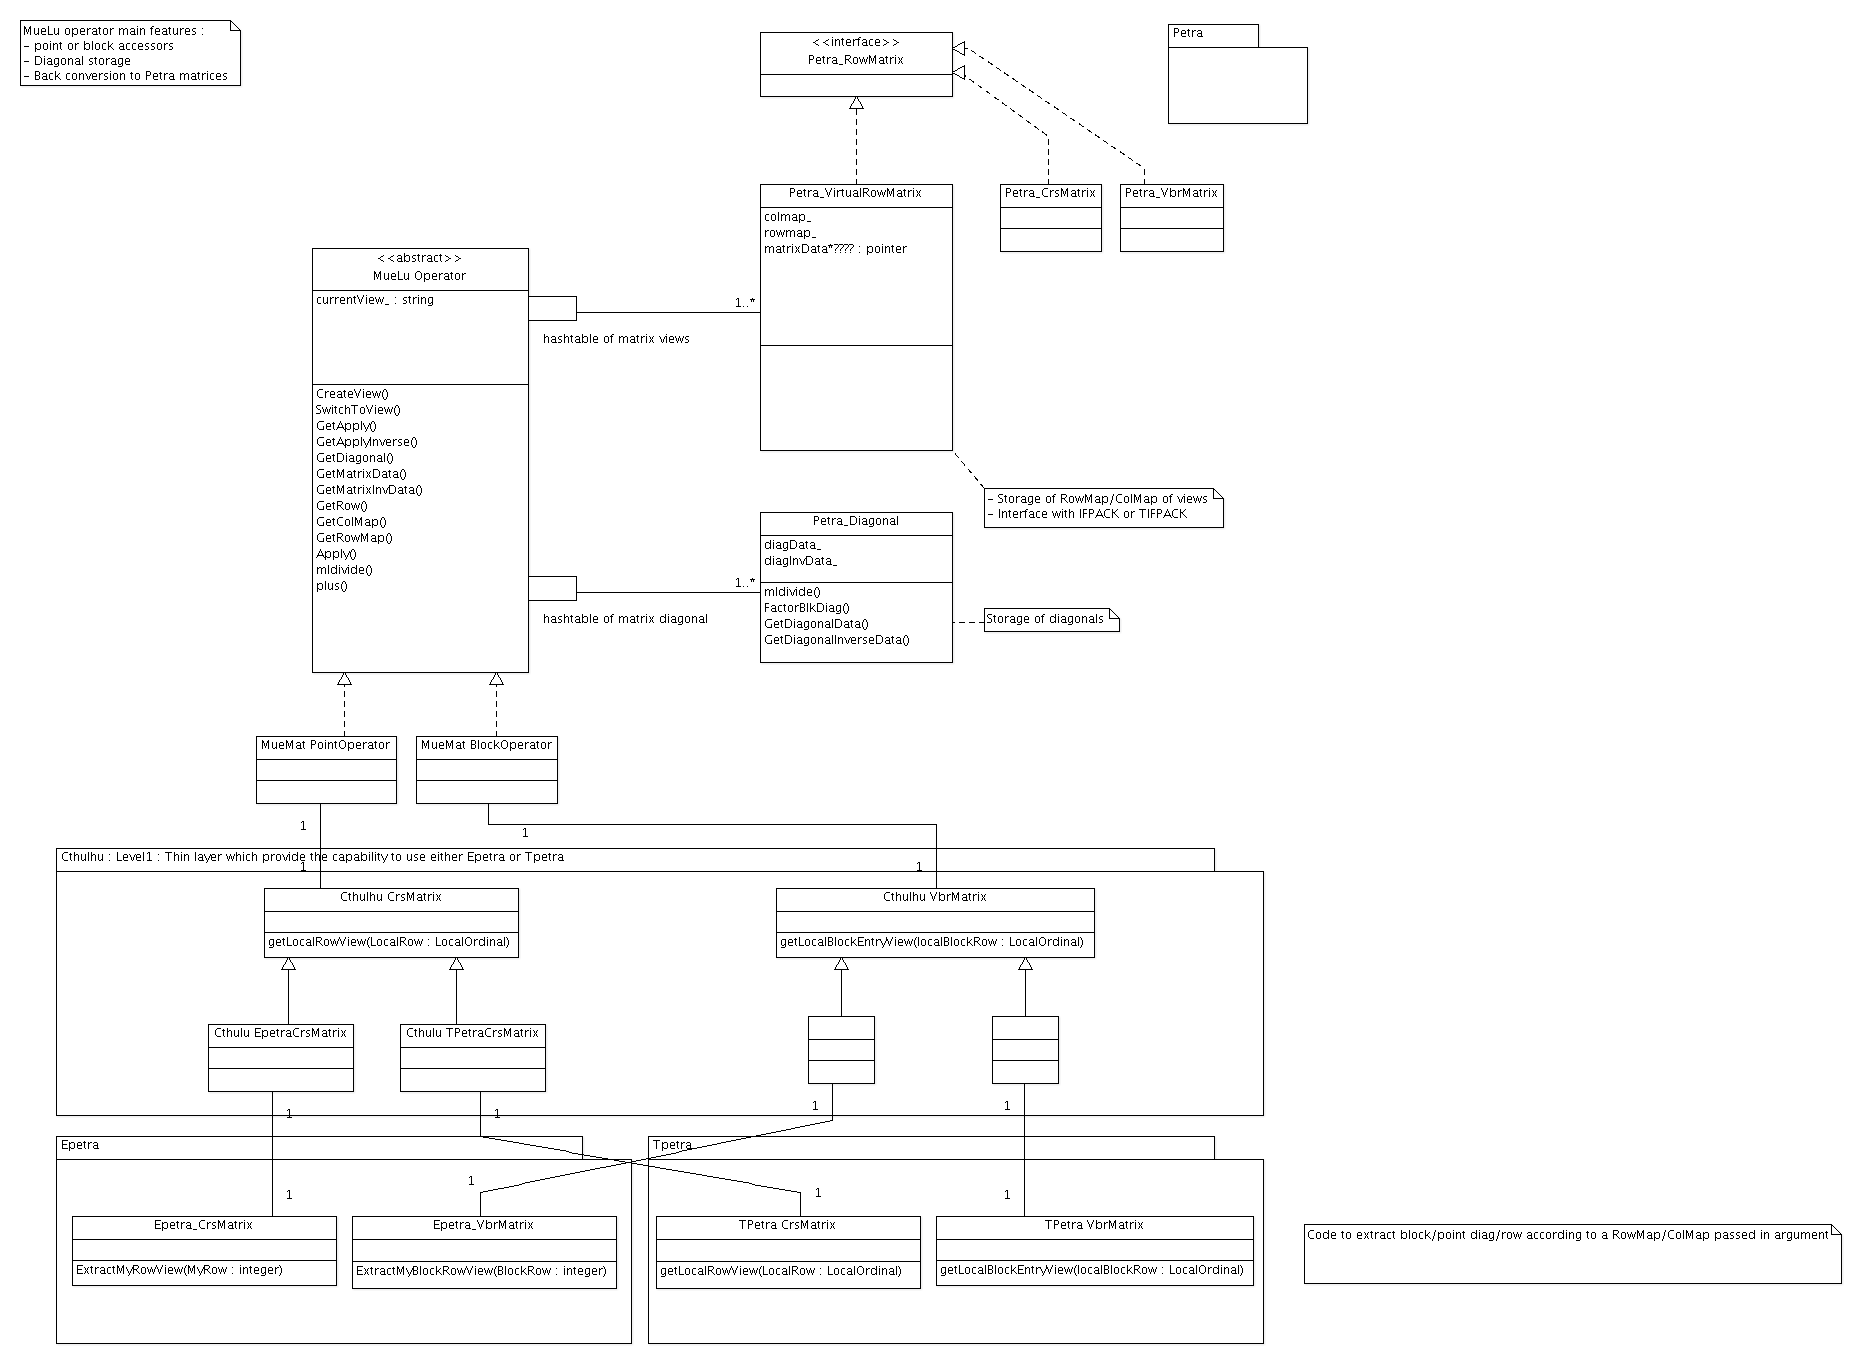
\includegraphics[angle=90,width=0.8\textwidth]{figs/MueLuOperatorClassDiagram.png}
  \caption{Class diagram of \Operator classes.}
  \label{fig:current:MueLuOperatorClassDiagram}
\end{figure}

\subsubsection{The \Operator class}
An \Operator is simply a matrix. In \muemat, the matrix data are natively stored as a MATLAB matrix (encapsulated in the \Operator object) and you can access directly to internal data storage by using the method GetMatrixData().
This accessor is used in \muemat for convenience and efficiency reasons.\\

In \mloo, matrices will be stored in \point or block form (using Epetra or Tpetra CsrMatrix or VbrMatrix). Such format provides row accessors (ie: GetRow() or GetBlockRow()):
\begin{itemize}
\item GetRow(i) returns the list of non-zeros of the row $i$ (as an array of columns indices and array of values).
\item GetRow(i) returns the list of blocks of the row $i$ (as an array of columns indices and an array of dense matrices).
\end{itemize}
In such format, matrix blocks are described by Map objects (\EpetraMap or \TpetraMap).\\

Some \muemat algorithms mimic the fact that we only have such row accessors: These algorithms loops over the rows and blocks and extract blocks from the MATLAB matrix:

\subsubsection{Additional remarks}

\begin{remark}
\label{prev}
A thin layer to be able to use easily Epetra or Tpetra matrix is also of interest for other projects than \mloo and should be available as a standalone library.
This implies to separate this functionality to other functionality of our future C++ \Operator class (and it implies
also to do more work to support all methods of Petra matrices).
\end{remark}

\begin{remark}
Same remark as remark \ref{prev} but for the multiview capability of our \Operator class. Such functionality should be added directly to petra libraries (by specializing CSR and VBR matrix classes).
\end{remark}

\subsubsection{The view mechanism}

One goal of the \Operator class is to be a thin interface layer between Epetra/Tpetra and \mloo (to allow us to be compatible with both libraries).


\subsection{Interface between the linear algebra packages (Epetra/Tpetra) and \mulu}

Why? - > compatible with Epetra and Tpetra

Should the linear algebra interface consist of:
\begin{itemize}
\item A single base class operator with view capabilities. This base class will be used in MueMat. Can derive specializations for each storage format.
\item ...
\end{itemize}

\subsubsection{Matrix-Matrix multiply used in MueMat}

$R A P = R (A P)$
\begin{enumerate}
\item point-point
\item point-block
\item block-block
\begin{itemize}
\item with the same block structure
\item $(I - D^{-1} A) P$ where $D^-1$ is $3\times3$, $A$ is $3\times3$ and $P$ is $3\times6$\\$\Rightarrow$ $(6\times3)$ multiplied by $(3\times3)$
\end{itemize}
\end{enumerate}

So, notion of compatible blocks... tbd

%3 mat-mat:
% pt-pt
% vbr-vbr -> convert to pt-pt (slow)
% block-block if compatible block.

$D^{-1} A$
\begin{itemize}
\item point-point
\item point-block
\item block-point
\item block-block
\end{itemize}


\subsubsection{Requirement}

Here are the summary of what we suppose to get from Epetra/Tpetra:

\begin{itemize}
\item Extraction of block diagonal and diagonal with overlap (Collection)
\item 
\end{itemize}

\subsubsection{Important issues}

Matrix-Matrix multiply in ?Petra.

\subsection{Interface between IFPACK/TIFPACK and \mulu}

A generic MueMat operator must be able to hand the underlying data to \Tifpack/\Ifpack/\AztecOO

\subsubsection{Important issues}
\begin{itemize}
\item \Tifpack smoothers currently always extract point diagonals.
\end{itemize}

\subsection{Summary of JG and JJH Discussion, 9/10/2010}

As a reminder, the view mechanism is the mechanism which allows someone to access a \mulu matrix as if it is stored using another data storage format. For instance, a point matrix can be access as a block matrix (via a \texttt{GetBlockRow} method) or vice versa. In addition, a 2x2 block matrix can also be viewed as a 4x4 matrix in \mulu. In this discussion, we suppose that the view mechanism is \textbf{not} provide by \Tpetra (or \TpetraExt) and is instead implemented either in \cthulhu\footnote{\cthulhu is our future linear algebra layer between EPetra/TPetra and \mulu} or \muelu.

There are essentially two paths that we can take to interface \mulu and \Tifpack.

\subsubsection{Path 1: \Tifpack and \muelu live in their own little worlds}

In the first path, we suppose that \Tifpack takes as arguments either \Tpetra point or block matrices, and provides (for both types of matrices) an implementation of point and block smoothers.

Here are some implications:

\be
\item \mulu\ must provide \Tpetra point/block matrices to \Tifpack (and other packages that use \Tpetra). In most cases, we can just pass to \Tifpack the internal matrix we stored.
  But, if we want to be able to use 4x4 block smoothers to 2x2 matrices, we need to provide \textbf{fake \Tpetra point/block matrices} to \Tifpack.
  Such fake matrices are just lightweight objects that respect the interface of \Epetra matrices and wrap method calls, i.e.,
  they derive from the {\tt Epetra\_RowMatrix} interface.

\item If \Tifpack is passed a {\tt Tpetra\_CrsMatrix}, but the user wants a block smoother, then \Tifpack has to do its own internal GetRow conversion to create blocks and apply the block smoother. There is potential code duplication between \mulu and \Tifpack concerning the mechanism to create blocks.

\item There is only one implementation of block smoothers in \Ifpack and this implementation is used for both point and block matrices. 
The block smoother is implemented using only the interface provided by \texttt{Epetra\_RowMatrix}. Indeed, \Ifpack uses the method \texttt{Epetra\_RowMatrix.ExtractMyRowCopy()} to build its own version of blocks.
The implementation of block smoothers for block matrices in \Ifpack is very inefficient. If the matrix is stored natively as a block matrix,
we should takes advantage of that in \Tifpack. In particular, a specicialized block smoother code must be written for block matrices.

\item Both \Tifpack and \muelu will need to extract (block) diagonals. Therefore, it make senses that \Tpetra (or \TpetraExt) provides a
method to extract \textbf{block} diagonals. This will avoid code duplication between \mulu and \Tifpack. We should also avoid extracting the
same diagonal more than once.

\ee

\subsubsection{Path 2: \Tifpack (and others) uses \cthulhu}

In this path, the view mechanism is implemented in \cthulhu. \Tifpack and \mulu use \cthulhu\ matrices.
Here are some implications:
\be
  \item The interface between \mulu and \Tifpack are simplified. We don't need anymore to create fake \Tpetra matrices. Other users of \Tifpack could provide \Tpetra matrices, which would immediately be wrapped as \cthulhu\ matrices at no cost.

  \item \Tifpack will use the view capabilities of \cthulhu. \Tifpack would not have to roll its own {\tt GetRow} and {\tt GetDiagonal} code.
  \item \Tifpack could provide efficient block relaxation schemes, etc., if the matrix is natively stored as a block matrix. We don't need an implementation for point matrices because point matrices can be viewed as block matrices.

  \item If \Tpetra (or \TpetraExt) doesn't provide a method to extract \textbf{block} diagonals, \cthulhu can provide it. In addition, we don't have to worry about multiple diagonal extraction because when the diagonal have been extracted, it is stored within the \cthulhu matrix.
\ee

\noindent Here are the main advantages if \Tifpack were to use \cthulhu:
\be
\item \Tifpack can now be used with  both \Epetra and \Tpetra matrices.
\item \Tifpack would not have to roll its own code to manage point and block matrices effectively (i.e.: dynamic cast of RowMatrix to CRSMatrix or VBRMatrix to avoid row copies when row views are enough; only one implementation of each smoother etc.). 
%\item Only one implementation of each smoothers is needed.

\item Any \Trilinos package, not just \muelu, can invoke \Tifpack with a blocking scheme other than the native one.
No additional code in \Tifpack is needed for this feature.
\ee

Note that we still can provide a mechanism to convert \cthulhu to fake Epetra/Tpetra matrices, but this functionality is now optional.%\footnote{In the path 2, we only need fake matrices for \Ifpack, if we want to be able to use 4x4 smoothers on 2x2 matrices using \Ifpack\dots}

\subsubsection{Commonalities}
%
\be
  \item \mulu\ will always use \cthulhu\ matrices internally.
  \item \cthulhu\ will always contain adapters to Epetra/Tpetra point and block matrices.
\ee

% Note: we will never convert Epetra matrices to TPetra matrices using the fake mechanism

\subsubsection{Implication of Path 1/2 to the class diagram}

In the first path, the \cthulhu layer can be dedicated to wrap Epetra/Tpetra matrices and to provide a common interfaces between these
libraries and \mulu. In this case, the \mulu\ Operator handles switching views. It contains the hashtables and the current view. Each view
will correspond to a particular row map (point or block), getrow, and diagonal. There are two implementations of the \mulu Operator
interface: one for matrices stored internally as CRS matrices and one for block matrices. There is no reason to push the view mechanism
down to \cthulhu if nobody uses it.

In the second path, \cthulhu\ handles switching of views.
So, the hashtable (\JG{or the whole MueMat operator ?}) gets pushed down to the \cthulhu\ level.
For example, suppose we have a \cthulhu\ EpetraCrsMatrix.  If in \mulu we want a block
view, we invoke a method in \cthulhu, which remembers this.\\
\JJH{This could have unintended side-effects if we're not careful.  The \cthulhu\ matrix state will persist, even when the matrix is
operated on by other Trilinos packages that use \cthulhu.}

\subsubsection{Discussion about advantage and drawback of each approach}

\begin{itemize}
\item Ray is concerned about the fact that Path~2 can slow down the development of \muelu (for example, if \Tifpack developers are waiting code from \cthulhu). This is certainly a valuable argument to take into account. Interaction between \mulu and \Tifpack will be more complicated in Path~2.
\item Path~2 have mostly advantages for TifPack developers and will be (ironically) more difficult to making accepted by \Tifpack developers (We force the use of \cthulhu !).
\item The amount of work for us is similar in both paths. In a coding perspective, the main difference between Path~1 and Path~2 is where the view mechanism is located (in \mulu or \cthulhu). 
If we decide to put the view mechanism in \cthulhu, we have the choice of moving from Path~1 to Path~2 in the future.
\item The mechanism to convert \cthulhu to fake Epetra/Tpetra matrices is not a critical feature. For \Tpetra/\Tifpack, we can directly pass the underlying \Tpetra matrices to \Tifpack (if \Tifpack smoothers are available for both TpetraCrsMatrix and TpetraVbrMatrix). The same is possible for the couple \Epetra/\Ifpack. In fact, fake matrices are required for:
\begin{itemize}
\item Applying block smoother with different blocking scheme than the native format of TpetraVbrMatrix (but only if \Tifpack don't have such functionality).
\item Using \Epetra matrices in \Tifpack or \Tpetra matrices in \Ifpack.
\end{itemize}
\item If \Tifpack don't use \cthulhu and don't provide an efficient block relaxation scheme for block matrices, we can roll our own later (and use \cthulhu in \Tifpack ourselves if it simplified developement).
\end{itemize}

Questions:
\begin{itemize}
\item What is the current state of \Tifpack ? Does \Tifpack developers plan to write an efficient block relaxation scheme for block matrices ? 
\item Do we need to plan a meeting with \Tifpack guys (at least to let them know about \cthulhu) ?
\item Path~1 or Path  2 ? Or we postpone the decision for the moment ?
\end{itemize}

\subsubsection{Chris' Comments}

\be
 \item Why does the serial matrix-matrix multiply that Ray will work on need to use \cthulhu?  Is this just to flesh out the \cthulhu\ API, or does the real
 multiply need to use \cthulhu?
 \item There is a 3rd path.  Namely, \cthulhu\ hides whether \Epetra or \Tpetra is being used.  Any block access, etc. is pushed down to the linear algebra
 level.  \JJH{My counter to this is that our pace of development is potentially constrained by what the \Tpetra/\Epetra developers want/specify/object
 to.}
\ee

\subsubsection{Ray's Comments}
Kernels for blocking

\be
\item We want to build a matrix graph associated with a block matrix even if
   the blocking does not match the original blocking in the matrix. This
   is useful for implementing Coalesce and it perhaps could be useful
   in a block matrix-matrix multiply. One good thing is that storage of
   the block matrix graph is often not too bad compared to the original
   matrix. For example, if we have a point matrix, the edge/vertex information
   would be relatively small for the associated block matrix graph 
   corresponding to something like 4x4 blocks, 

\item We want something like GetBlockRow(). This is relatively easy if we have
   a point matrix. It is somewhat more costly if we have a block matrix
   and we want to get a point row. This involves first figuring out which
   block row contains a point row. We could actually store something to
   make this fast. Then, there are a bunch of offsets to figure out 
   for each nonzero block in this block row (and of course none of the
   data is contiguous).

\item A bit more tricky is that the matrix-matrix multiply might want to
   easily get a sub-block within a Block Row. This would implies that
   GetBlockRow() should really return a list of blocks. If the underlying
   format is a point matrix, this would mean copy data and reorganizing
   it into a list of blocks. One might be able to make this okay efficient
   if the block matrix graph is stored ... perhaps with a little auxilliary
   info.

\item This might mean that it would be useful to have cThUlHu commands to
   build auxilliary information to optionally make something more efficient 
   and perhaps special commands to remove this auxilliary information 
   if it is not needed.
\ee

At the lowest level, it looks like we want something like
\be
   \item BuildBlockGraph(Matrix,RowMap,ColMap) perhaps with some way to efficiently include dropping? 
   \item GetRow(Matrix,Row) 
   \item GetBlockRow(Matrix,BlkRow) which returns a list of blocks
   \item MatVec
   \item SubsetMatVec
   \item OptimizeForGetBlockRow(Matrix)
   \item RemoveOptimization(Matrix)
   \item GetDiag(Matrix)
   \item GetBlkDiag(Matrix)
\ee
I would guess that SubsetMatVec() in conjunction with GetBlkDiag() is a more
efficient way to implement Gauss-Seidel than GetBlockRow().

We probably also need things like NNZ() and MaxNNZPerRow(). We might need 
these to work in a block sense?

Parallel?
